\chapter{Procesos}
\begin{BPMN}{PROC-01}{Creación de un Programa Académico}{}
    \PCitem{Participantes}{Unidad Académica, DES, Consejo General Consultivo y Direccion General}
    \PCitem{Objetivo}{La elaboración o renovación de los Programas Académicos  del IPN, partiendo desde el análisis de la propuesta, la elaboración del plan de estudios hasta la conformación del mapa curricular y las unidades de aprendizaje, siendo revisado en cada etapa por las autoridades correspondientes}
    \PCitem{Interrelación con otros procesos}{}
    \PCitem{Proveedores}{Agentes internos o externos del IPN}
    \PCitem{Entradas}{Propuesta de creación o renovación de programa académico}
    \PCitem{Consumidores}{Unidad Académica, DES, Consejo General Consultivo y Direccion General}
    \PCitem{Salidas}{Programa académico}
    \PCitem{Precondiciones}{Solicitud de nuevo programa académico}
    \PCitem{Postcondiciones}{Aplicacion del nuevo programa academico}
    \PCitem{Frecuencia}{}
    \PCitem{Tipo}{Operativo}
    \PCitem{Áreas de oportunidad}{Registro y revisión de planes de estudio, mapas curriculares y unidades de aprendizaje en línea }
\end{BPMN}
En la figura \hyperref[]{}
\begin{figure}[htbp]
	\begin{center}
		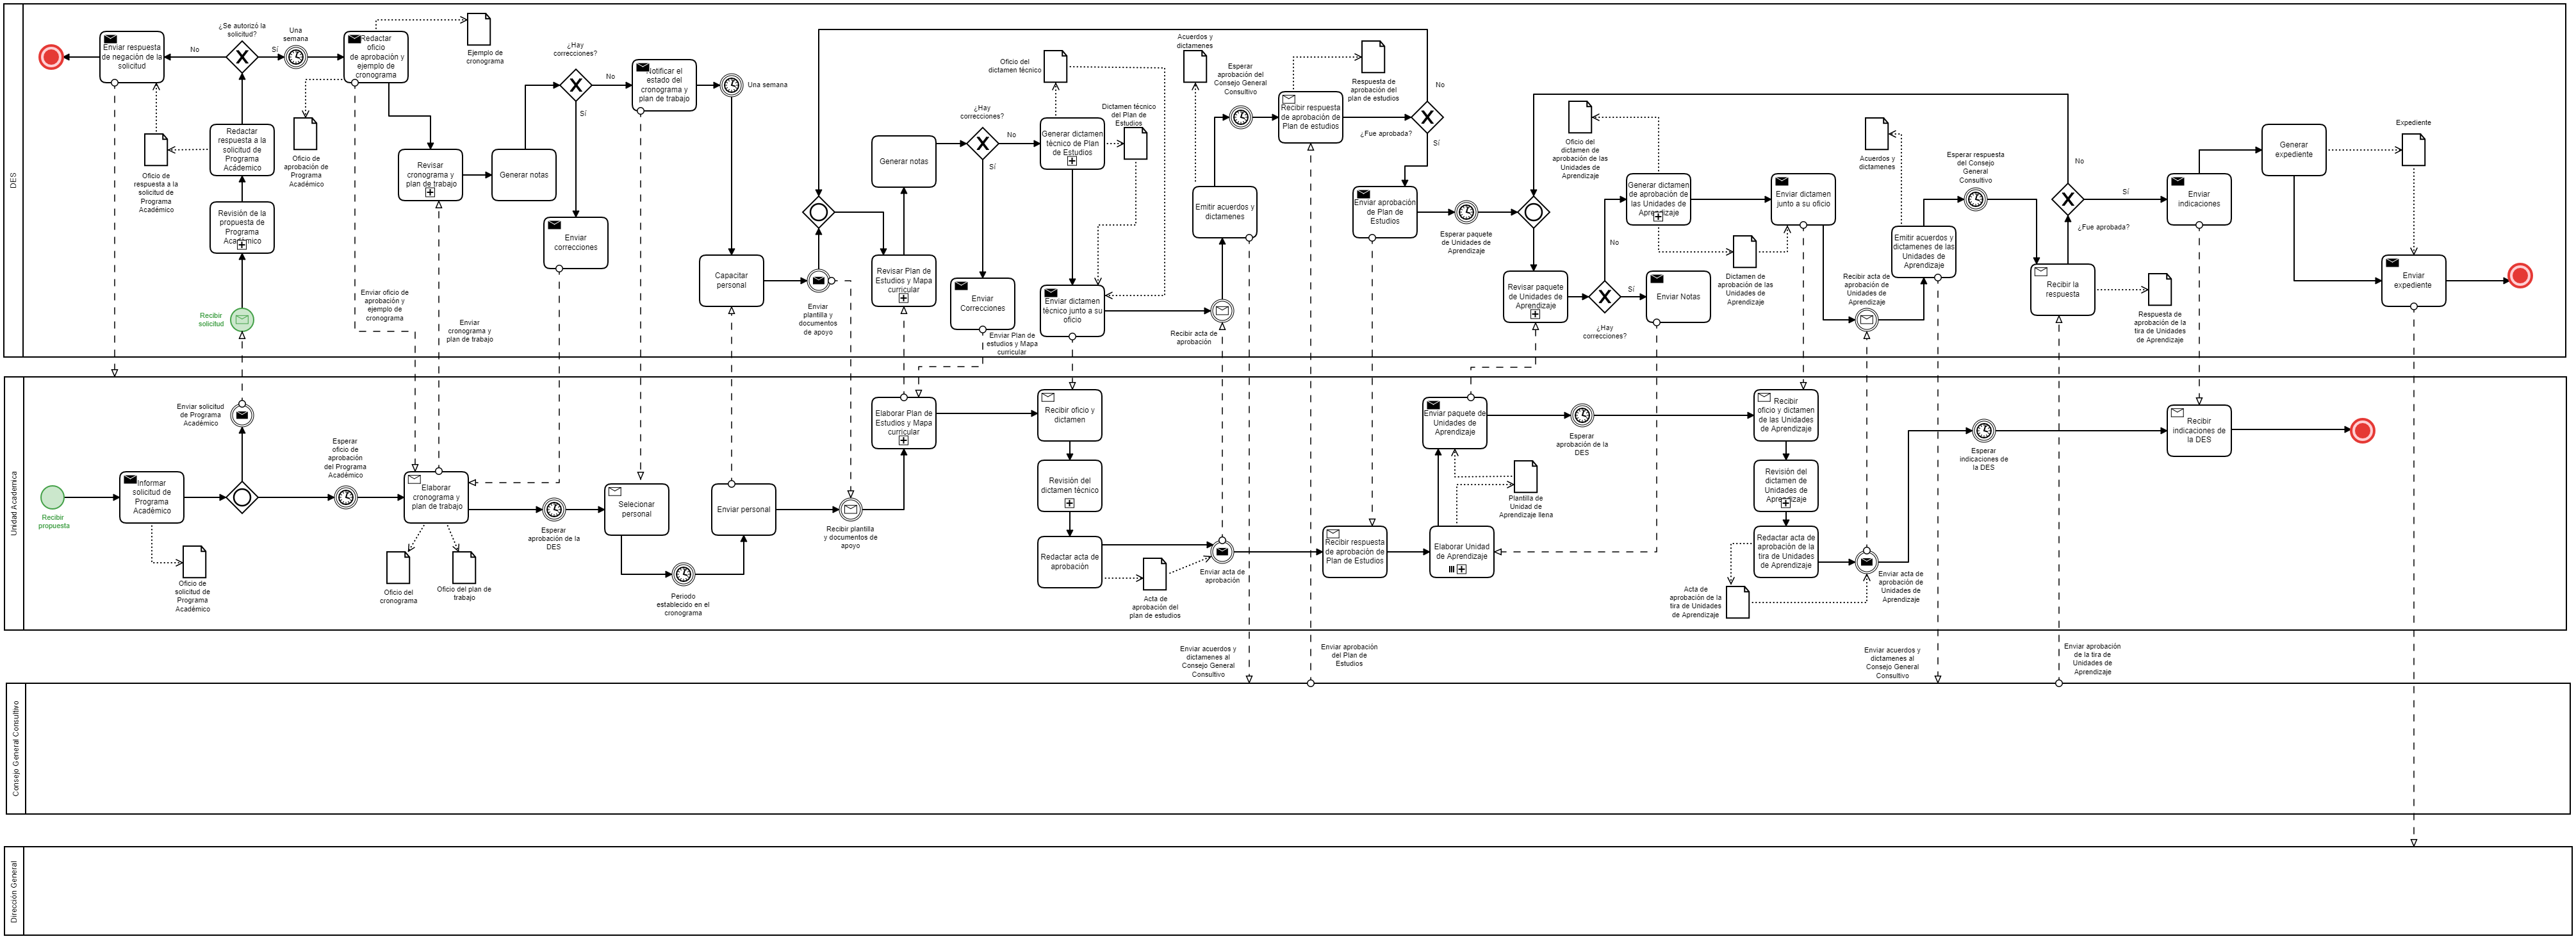
\includegraphics[width=.95\textwidth]{C1-DP/MP/bpmnMacro.png}
		\caption{}
		\label{fig:}
	\end{center}
\end{figure}